\documentclass[10pt,a4paper]{article}
\usepackage[utf8]{inputenc}
\usepackage{amsmath}
\usepackage{amsfonts}
\usepackage{amssymb}
\usepackage{subcaption}
\usepackage{longtable}
\usepackage[section]{placeins}
\usepackage{graphicx}
\usepackage{xcolor}
\usepackage[numbers]{natbib}
\author{Ignace Bleukx \and Quinten Bruynseraede}
\title{Machine Learning Project: part 1}

\addtolength{\oddsidemargin}{-.875in}
\addtolength{\evensidemargin}{-.875in}
\addtolength{\textwidth}{1.75in}
\addtolength{\topmargin}{-.875in}
\addtolength{\textheight}{1.75in}
\begin{document}
\maketitle

\section{Literature Review}
In this first assignment we try to combine basic principles from game theory with the work concerning multi-agent reinforcement learning. Most literature included in this literature review will therefore more or less fall into one of these categories. First we give an overview of the relevant literature, along with their contributions.


\bigskip
\begin{longtable}{|p{4cm}|p{12cm}|}
\hline 
Article & Contribution \\ 
\hline 
\hline
Multi-agent systems: Algorithmic, Game-Theoretic, and Logical Foundations, \citet{mas} & This paper provides a thorough explanation of the different aspect of game theory, including different types of equilibria. These concepts are of importance to us since we will investigate whether or not our learning algorithms converge to one of these equilibria. Furthermore, the paper provides a detailed description of different types of games, such as cooperative games and non-cooperative games, as well as the notion of games in normal form.   \\ 
\hline 
Multi-agent learning dynamics, \citet{phdthesis} &  This thesis on multi agent learning dynamics provides essential information about different game theoretic aspects. Mainly section 2.3 on evolutionary game theory and chapter 3 on learning dynamics are relevant. In this last chapter, the replicator dynamics of many matrix games are investigated and explained very clearly. In this chapter we find an example of the learning pattern we would like to observe with our application of different learning algorithms.   \\
\hline 
OpenSpiel: A Framework for Reinforcement Learning in Games, \citet{lanctot2019openspiel} & The paper provides the documentation of the OpenSpiel framework. All aspects of the library are explained, from installation to implemented algorithms and games. Many design choices of the framework are clarified which helps to understand the philosophy behind the framework. In the paper, the game theoretic aspects are briefly touched, as well as important concepts of the implemented learning algorithms. This paper is of very much importance to us as we will use (and potentially extend) the OpenSpiel framework for this assignment. \\ 
\hline  
Reinforcement learning produces dominant strategies for the Iterated Prisoner’s Dilemma, \citet{rlforpd} & 
This document contains a detailed description of the prisoners dilemma, which we will examine. Some examples of parameters settings for the training algorithms are given, which will help to produce meaningful results when training the learning algorithms of choice.\\ 
\hline 
The replicator equation on graphs, \citet{Ohtsuki2006TheRE} & This paper provides an insight on the visualization of the replicator dynamics using phase plots, as well as some examples relevant to our research. These examples include the prisoners dilemma and biased rock-paper-scissors.\\
\hline
Analyzing Reinforcement Learning algorithms using Evolutionary Game Theory, \citet{bloembergenmaster} & This thesis provides a rich source of information on the reinforcement learning branch of evolutionary game theory. Many algorithms are examined, some of which are available in OpenSpiel. The paper also contains the exact parameter settings used to reproduce its results. These parameters can be used by our agents to achieve similar results. \\
\hline
Evolutionary Dynamics of Multi-Agent Learning:A Survey, \citet{evoldynamics} & Like other papers, this document provides a basic knowledge of game theory, as well as reinforcement learning. For our research, mainly the part about lenient FAQ-learning as a way to increase the robustness of Q-learning, is important. FAQ-learning is able to recover from bad exploration in the start of the run, while normal Q-learning is sometimes not. \\
\hline
Extended Replicator Dynamics as a Key to Reinforcement Learning in Multi-agent Systems, \citet{extrepl} & To model stochastic policies, populations of players are used. These populations can be described using evolutionary concepts, such as selection and mutation. This paper explains the transition from regular to evolutionary game theory. We received insight on the dynamics of a population through the central notion of replicator dynamics. These selection mechanisms can be extended with mutation, based on the Boltzmann mechanism. To overcome converge to suboptimal equilibria, lenience towards mistakes is introduced in this paper.
\\ 
\hline
\end{longtable} 

\section{Independent learning}
\begin{figure}[h]
    \centering
    \begin{subfigure}[b]{0.33\textwidth}
        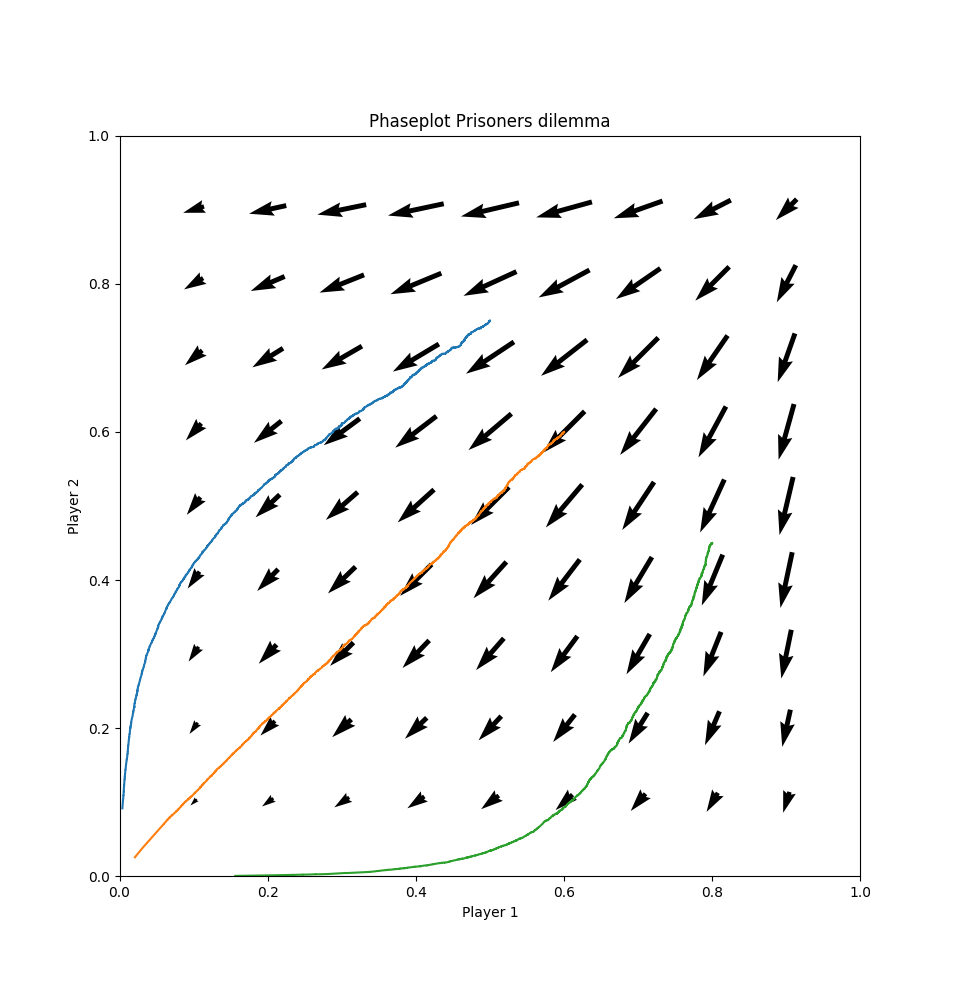
\includegraphics[width=\textwidth]{Figures/cl_pd.png}
    		\caption{Prisoner's dilemma}
    \end{subfigure}
    \begin{subfigure}[b]{0.33\textwidth}
        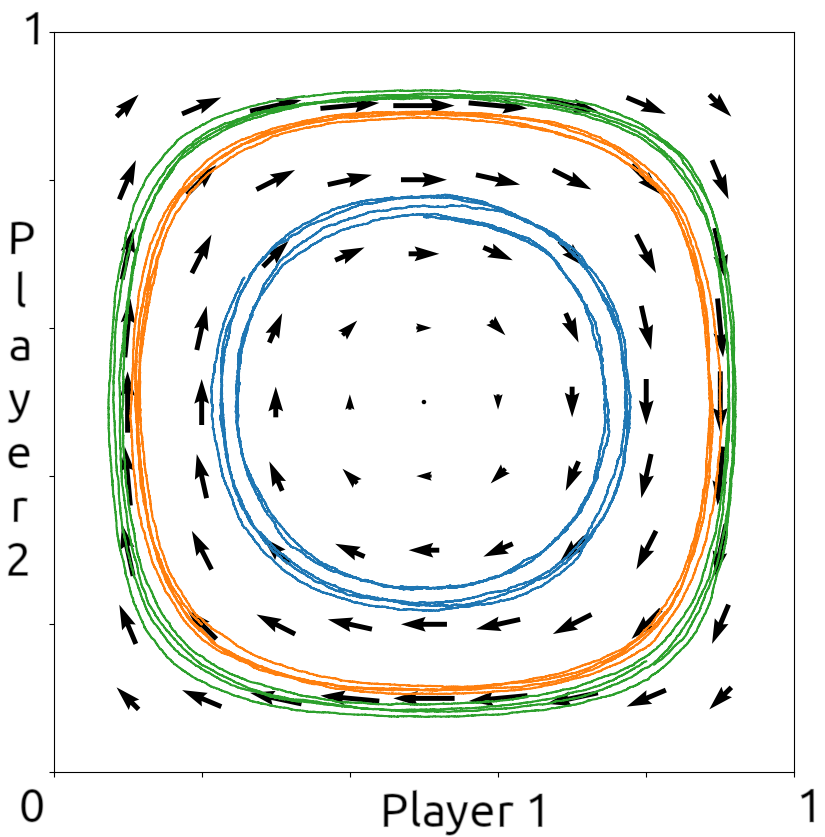
\includegraphics[width=\textwidth]{Figures/cl_mp.png}
        \caption{Matching Pennies}
    \end{subfigure}
    \begin{subfigure}[b]{0.33\textwidth}
        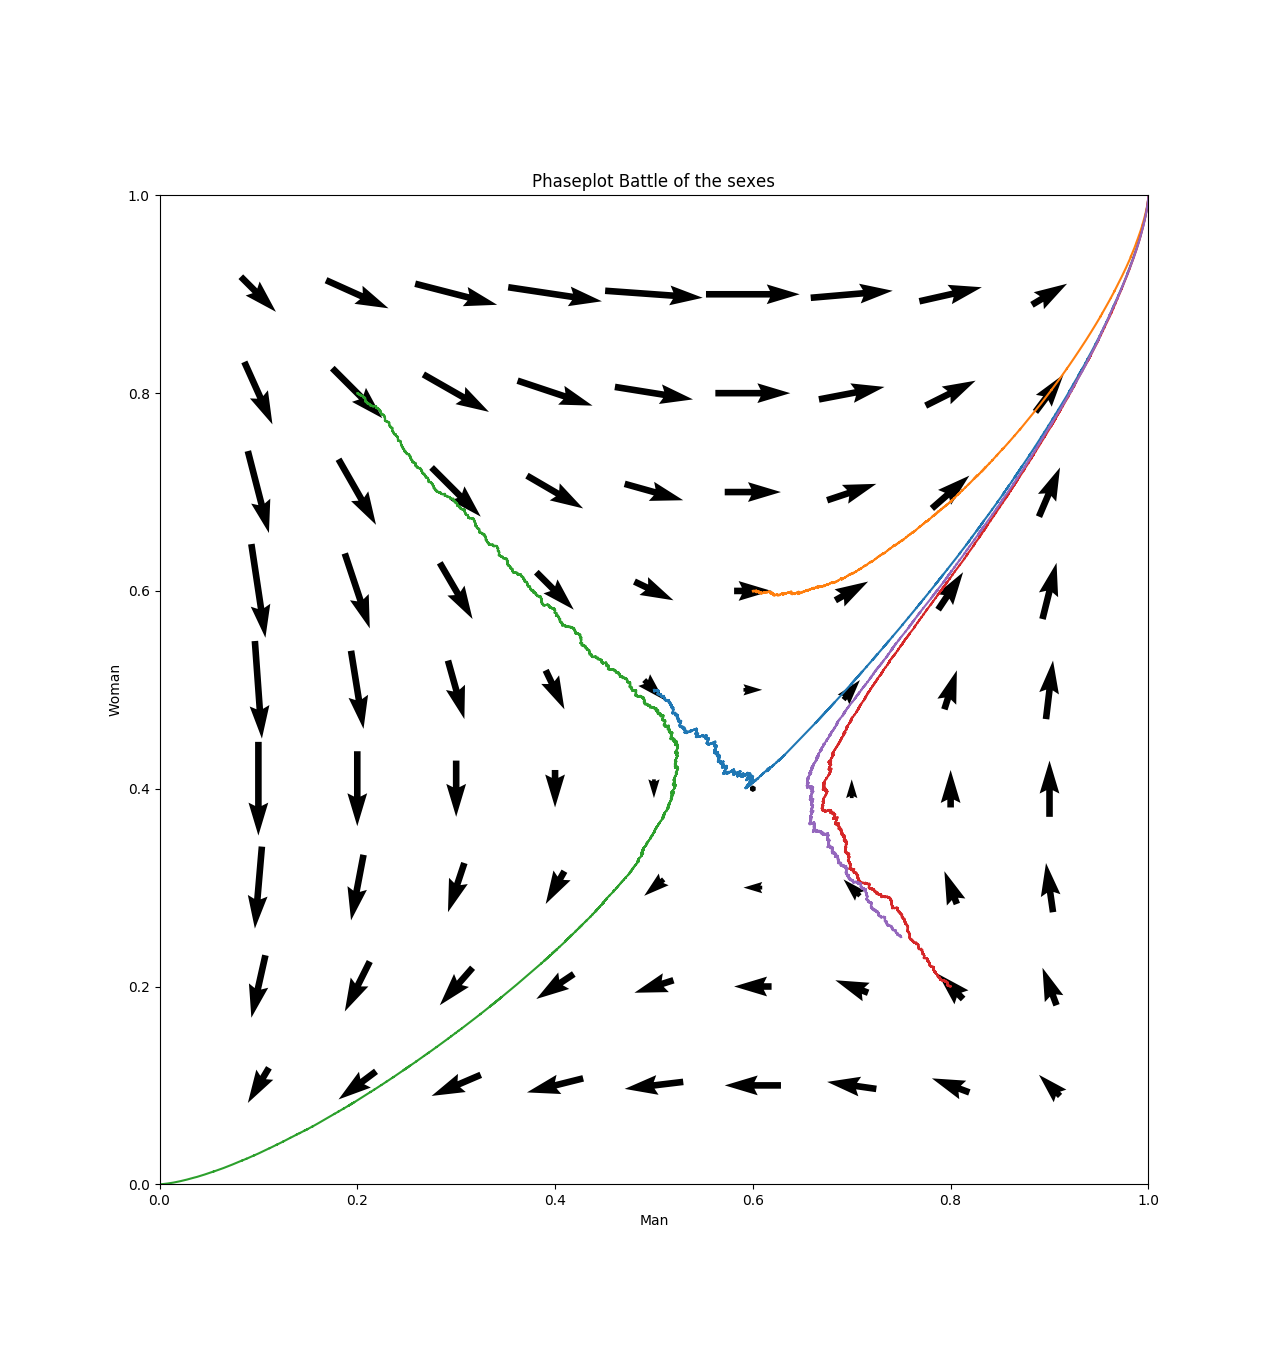
\includegraphics[width=\textwidth]{Figures/cl_bots.png}
        \caption{Battle of the Sexes}
    \end{subfigure}
    \begin{subfigure}[b]{0.33\textwidth}
        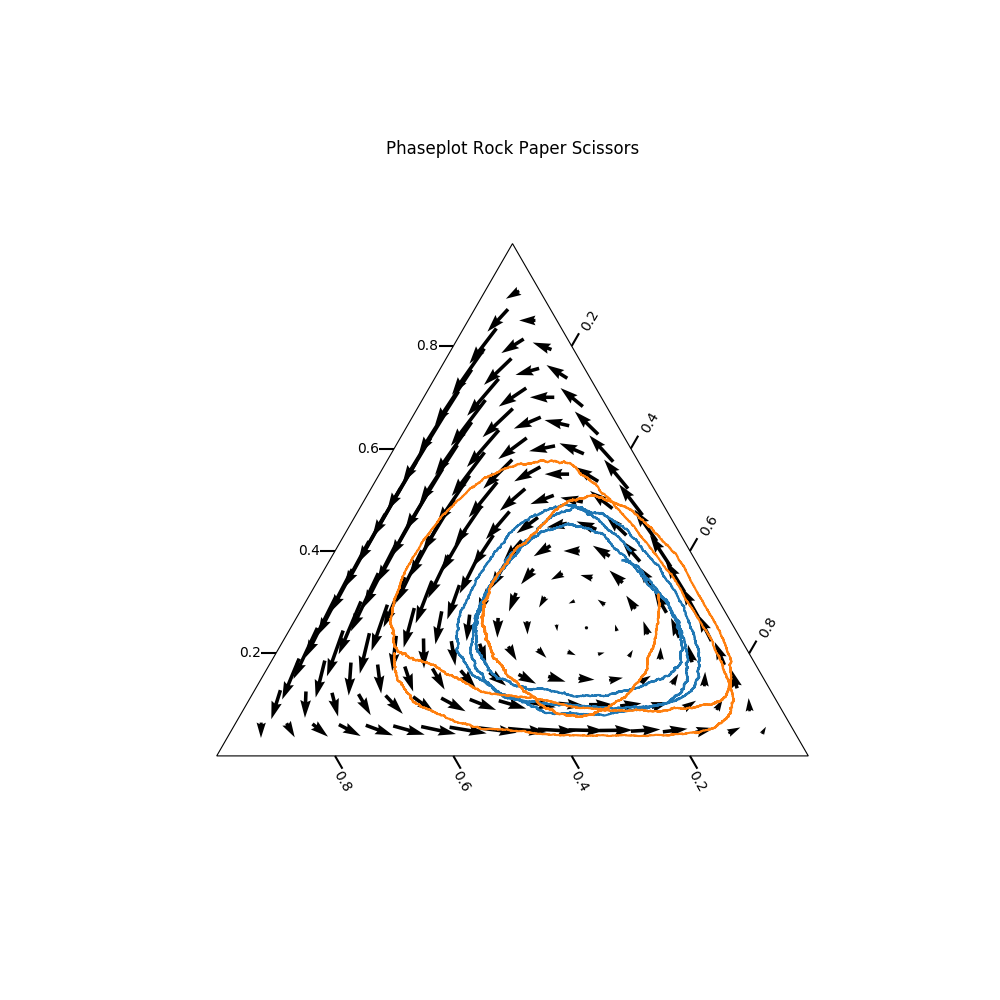
\includegraphics[width=\textwidth]{Figures/cl_rps.png}
        \caption{Biased Rock Paper Scissors} 
    \end{subfigure}
    \label{fig:learning}
    \caption{Learning trajectories in benchmark games}
\end{figure}

For this section we implemented our own reinforcement learning agent which follows the \textit{Cross Learning} algorithm. B\"{o}rgers \& Saring were the first to formally show the relationship between multi-agent learning and evolutionary game theory by proving that Cross Learning converges to the replicator dynamics when the agent's step size goes towards 0. For this reason, we chose to implement Cross Learning: we can expect its learning trajectories to follow our directional plot more or less exactly. In Figure 1, we show how our algorithm learns four games: the prisoner's dilemma, the matching pennies game, the battle of the sexes, and biased Rock-Paper-Scissors. Also included in Figure 1 are the directional phase plots for replicator dynamics. Each plot contains learning trajectories from multiple initial policies.\\


Cross Learning converges to $(0,0)$ for the Prisoner's Dilemma, the situation in which both prisoners defect. This is a Nash equilibrium, as both players will lower their reward by cooperating while the other player still defects. It is also Pareto optimal, because when one player suddenly decides to cooperate, he himself receives a lower reward. It is therefore not possible to improve a strategy without lowering the reward for another player.\\

In the Matching Pennies game, the algorithm converges to $(\frac{1}{2},\frac{1}{2})$, which is a Nash equilibrium: if a player decides to change his strategy whilest the other one keeps playing heads or tails randomly, he will be at a disadvantage. As Matching Pennies is a zero-sum game, all strategies are Pareto-optimal: there is a set amount of reward to distribute, so improving a player's reward lowers the reward for another player.\\

A known result from Game Theory is that the Battle of the Sexes games has three equilibria, one of which is mixed. The strategies $(1,1)$ and $(0,0)$ are pure Nash equilibria, while $(\frac{3}{5},\frac{2}{5})$ is a mixed Nash equilibrium. $(1,1)$ and $(0,0)$ are Pareto optimal, because changes in policies have the following effects: when one player changes his strategy, both players go to a different activity and receive no reward. When both players change their strategy, one player doesn't go to his preferred activity anymore. The mixed strategy is also Pareto optimal: going to your preferred solution more often lowers the reward of your partner, etc. This mixed strategy is unstable.\\

For the Biased Rock Paper Scissors game, we observe one equilibrium in the directional phase plots, at approximately $(\frac{1}{4},\frac{2}{4},\frac{1}{4})$. Regular Rock Paper Scissors has its Nash equilibrium at $(\frac{1}{3},\frac{1}{3},\frac{1}{3})$, but changing the payoff matrix moves this equilibrium towards a certain action. As Rock Paper Scissors is essentially Matching Pennies with three actions, it is a zero-sum game. Therefore, any strategy profile is Pareto optimal, using the same argument as before.

All experiments were executed for 30 000 iterations, a learning rate of 0.001. To demonstrate the correlation between Cross Learning and replicator dynamics, we did not average out results of multiple experiments. Instead, we kept the learning rate as low as possible.

\section{Dynamics of learning}

\subsection{Lenient Boltzmann Q-Learning dynamics}
Based on \citet{evoldynamics}, we implemented Lenient Boltzmann Q-Learning dynamics. This extension introduces two parameters. The first parameter, $\kappa$, is the degree of leniency: the number of rewards that are examined in each step before updating the policy. We expect to see improved robustness when introducing leniency. Intuitively, this is done by increasing the area of attraction for optimal equilibria. Secondly, $\tau$ introduces entropy into the population: a learner will favour exploration over exploitation when $\tau$ increases. We expect fixed points of the dynamics to stray away from Nash equilibria as $\tau$ is increased. However, introducing a small amount of entropy may prevent attraction from unwanted equilibria early on.

\begin{figure}[h]
    \centering
    \begin{subfigure}[b]{0.30\textwidth}
        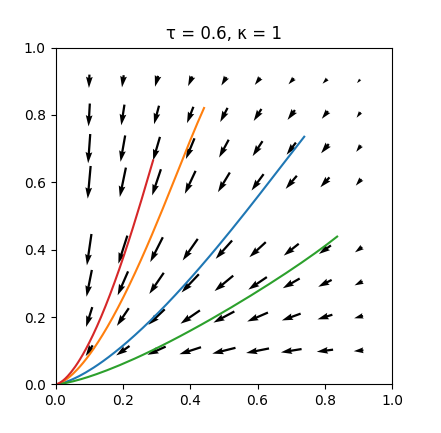
\includegraphics[width=\textwidth]{Figures/boltzmann_pd_1.png}
    \end{subfigure}
    \begin{subfigure}[b]{0.30\textwidth}
        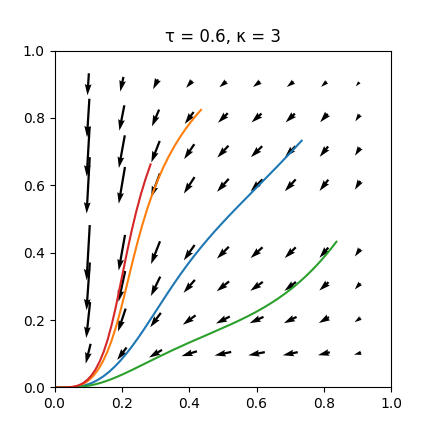
\includegraphics[width=\textwidth]{Figures/boltzmann_pd_3.png}
    \end{subfigure}
    \begin{subfigure}[b]{0.30\textwidth}
        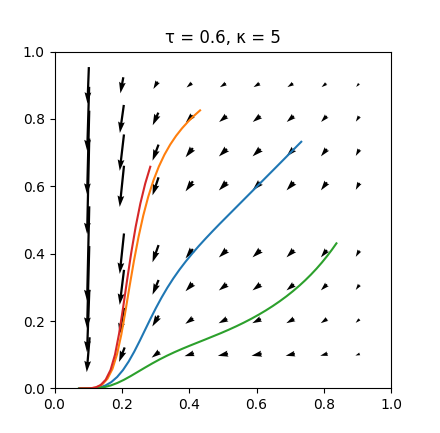
\includegraphics[width=\textwidth]{Figures/boltzmann_pd_5.png}
    \end{subfigure}
    \caption{LFAQ for the Prisoner's dilemma}
    \vspace*{-10mm}
    \label{fig:boltz_pd}
\end{figure}
\begin{figure}[h]
    \centering
    \begin{subfigure}[b]{0.30\textwidth}
        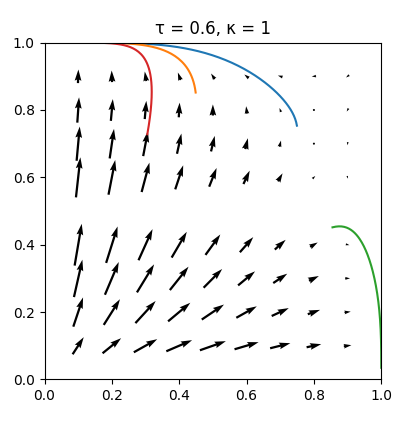
\includegraphics[width=\textwidth]{Figures/boltzmann_bots_1.png}
    \end{subfigure}
    \begin{subfigure}[b]{0.30\textwidth}
        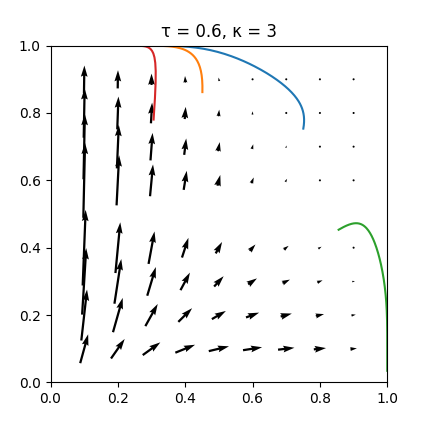
\includegraphics[width=\textwidth]{Figures/boltzmann_bots_3.png}
    \end{subfigure}
    \begin{subfigure}[b]{0.30\textwidth}
        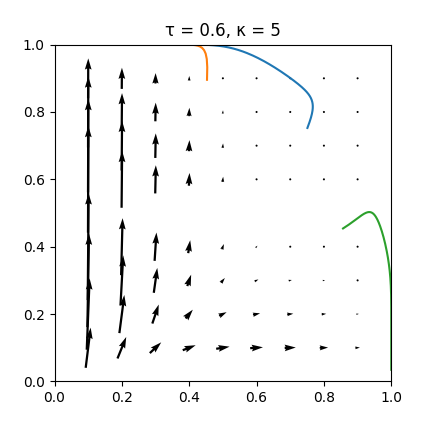
\includegraphics[width=\textwidth]{Figures/boltzmann_bots_5.png}
    \end{subfigure}
    \caption{LFAQ for the Battle of the Sexes}
    \vspace*{-10mm}
    \label{fig:boltz_bots}
\end{figure}
\begin{figure}[h]
    \centering
    \begin{subfigure}[b]{0.30\textwidth}
        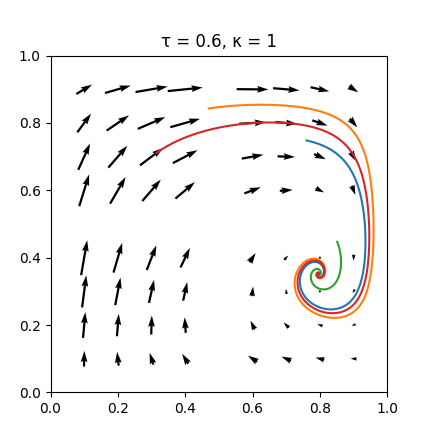
\includegraphics[width=\textwidth]{Figures/boltzmann_mp_1.png}
    \end{subfigure}
    \begin{subfigure}[b]{0.30\textwidth}
        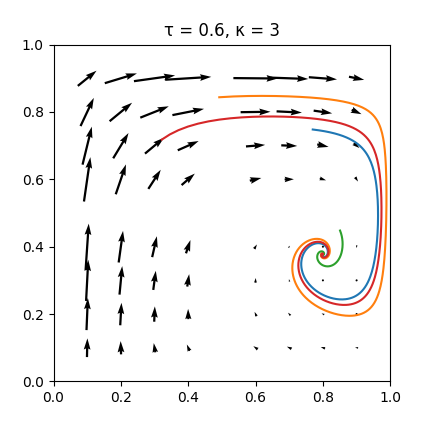
\includegraphics[width=\textwidth]{Figures/boltzmann_mp_3.png}
    \end{subfigure}
    \begin{subfigure}[b]{0.30\textwidth}
        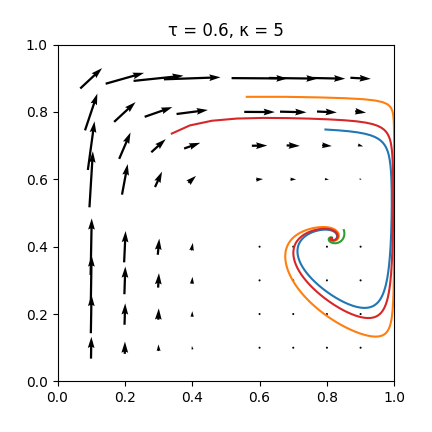
\includegraphics[width=\textwidth]{Figures/boltzmann_mp_5.png}
    \end{subfigure}
    \caption{LFAQ for the Matching Pennies game}
    %\vspace*{-10mm}
    \label{fig:boltz_mp}
\end{figure}

Figures \ref{fig:boltz_pd} through \ref{fig:boltz_mp} show the influence of the parameter $\kappa$ on the dynamics. For games such as the Prisoner's Dilemma with one equilibrium (in this case located at 0,0), the difference isn't very interesting. However, in Figure \ref{fig:boltz_bots}, we clearly see how there is no longer attraction to the suboptimal equilibrium at ($\frac{3}{5}$,$\frac{2}{5}$).
\\

The influence of $\tau$ is very clear, as shown in Figure \ref{fig:tau}. As $\tau$ increases, exploration of new solutions is greatly preferred. Therefore, an agent will not further capitalize on improvements in his strategy. As a result, policies seem to converge to random guessing. A small of amount of entropy, however, may increase robustness of a learner.


\begin{figure}[h]
    \centering
    \begin{subfigure}[b]{0.30\textwidth}
        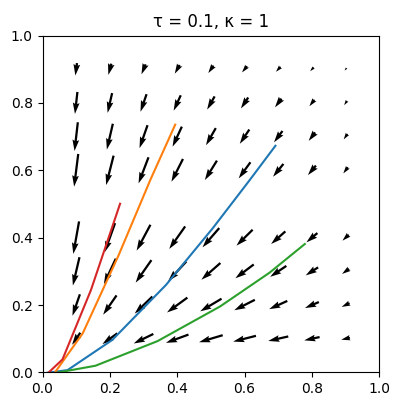
\includegraphics[width=\textwidth]{Figures/boltzmann_pd_temp01.png}
    \end{subfigure}
    \begin{subfigure}[b]{0.30\textwidth}
        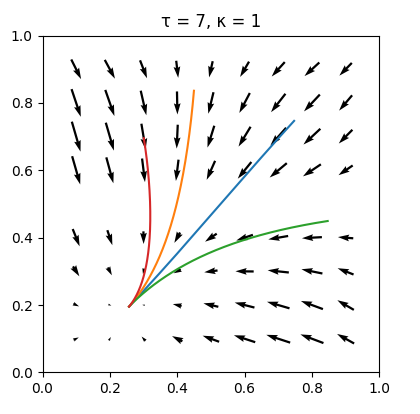
\includegraphics[width=\textwidth]{Figures/boltzmann_pd_temp7.png}
    \end{subfigure}
    \begin{subfigure}[b]{0.30\textwidth}
        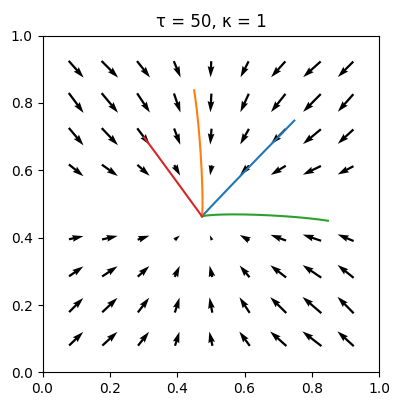
\includegraphics[width=\textwidth]{Figures/boltzmann_pd_temp50.png}
    \end{subfigure}
    \caption{Influence of increasing $\tau$ on the Prisoner's Dilemma}\label{fig:tau}
\end{figure}

\section{Part 2 and 3}
The task in parts 2 and 3 are similar: train an agent to play both games. We will start of by applying some standard tabular learner to the problem, e.g. Cross Learning or Q-Learning. At some point (mostly for Leduc Poker), we will run into practical limits for tabular learners. This is where we explore approximation through neural networks. Deciding which features of the information state to use will be crucial. To improve performance, we will look into approximating hidden features (the opponent's cards). \citet{poker} can be a starting point for this part. When we run into the practical limits of these approximation methods, improving the efficiency of our learning architecture can be examined. \citet{dulacarnold2015deep} propose a tractable learning strategy that scales linearly in the number of actions. Their 'related work' section outlines some other strategies to improve the scalability of training reinforcement learning agents in the context of games. 

\bibliography{lit}{}
\bibliographystyle{plainnat}

\section*{Appendix}
The payoff matrix for the biased Rock-Paper-Scissors game is given below:
\begin{center}
\begin{tabular}{|c|c|c|c|}
\hline
& Rock & Paper & Scissors \\ \hline
Rock & 0,0 & -1,1 & 2,-2 \\ \hline
Paper & 1,-1 & 0,0 & -1,1 \\ \hline
Scissors &-2,2 & 1,-1 & 0,0 \\ \hline
\end{tabular}
\end{center}

\end{document}

